% !TeX root = ./corona_contact_tracing.tex
% chktex-file 46
% !TeX spellcheck = en-GB
% !TeX encoding = utf8

\section{Algorithm notes}

\subsection{SIR Model}
Our basic stochastic SIR model relies on the assumptions that every person in an environment can be modeled as a point value, which has a location (i.e.\ GPS coordinates) and an infection state. These states can be either \textit{susceptible} (S), \textit{infected} (I), \textit{recovered} (R) or in advanced models also \textit{under quarantine} (Q) or \textit{dead} (D). All individuals, here called agents, have a probability (here called diffusion rate $d$ to make a step per time step on a predefined grid. In the case, that some agents meet at the same location, disease spreading can occur. An infected agent spreads the disease with probability $\beta$ to all the agents in its close vicinity (same location on the grid). Furthermore recovery is covered by taking a recovery rate into account, i.e a probability $\gamma$ to recover from the disease per time step. If an infected agent recovers from the disease, the state of the agent changes from \textit{infected} to \textit{recovered}, which is definite (no double infections). The process ends, when no infected agents are left.
\begin{center}
    Susceptibles $\overset{\beta}{\longrightarrow}$ Infected $\overset{\gamma}{\longrightarrow}$ Recovered.
\end{center}

An example of a early model state is shown in Figure~\ref{fig:1}
\begin{figure}[H]
    \centering
    \includegraphics[width=0.4\linewidth]{initial_setup.png}
    \caption{Early state of SIR model, blue dots = susceptibles, red dots = infected agents, green dots = Recovered agents}%
    \label{fig:1}
\end{figure}

In this case, 1000 agents were initialized on a 100 by 100 grid, where a certain amount of infected agents were introduced as a seed. Letting the agents perform random walks on the grid (maximally one step each time step with probability $d$), and letting the model converge, the results in figure~\ref{fig:2} can be observed.

\begin{figure}[H]
    \centering
    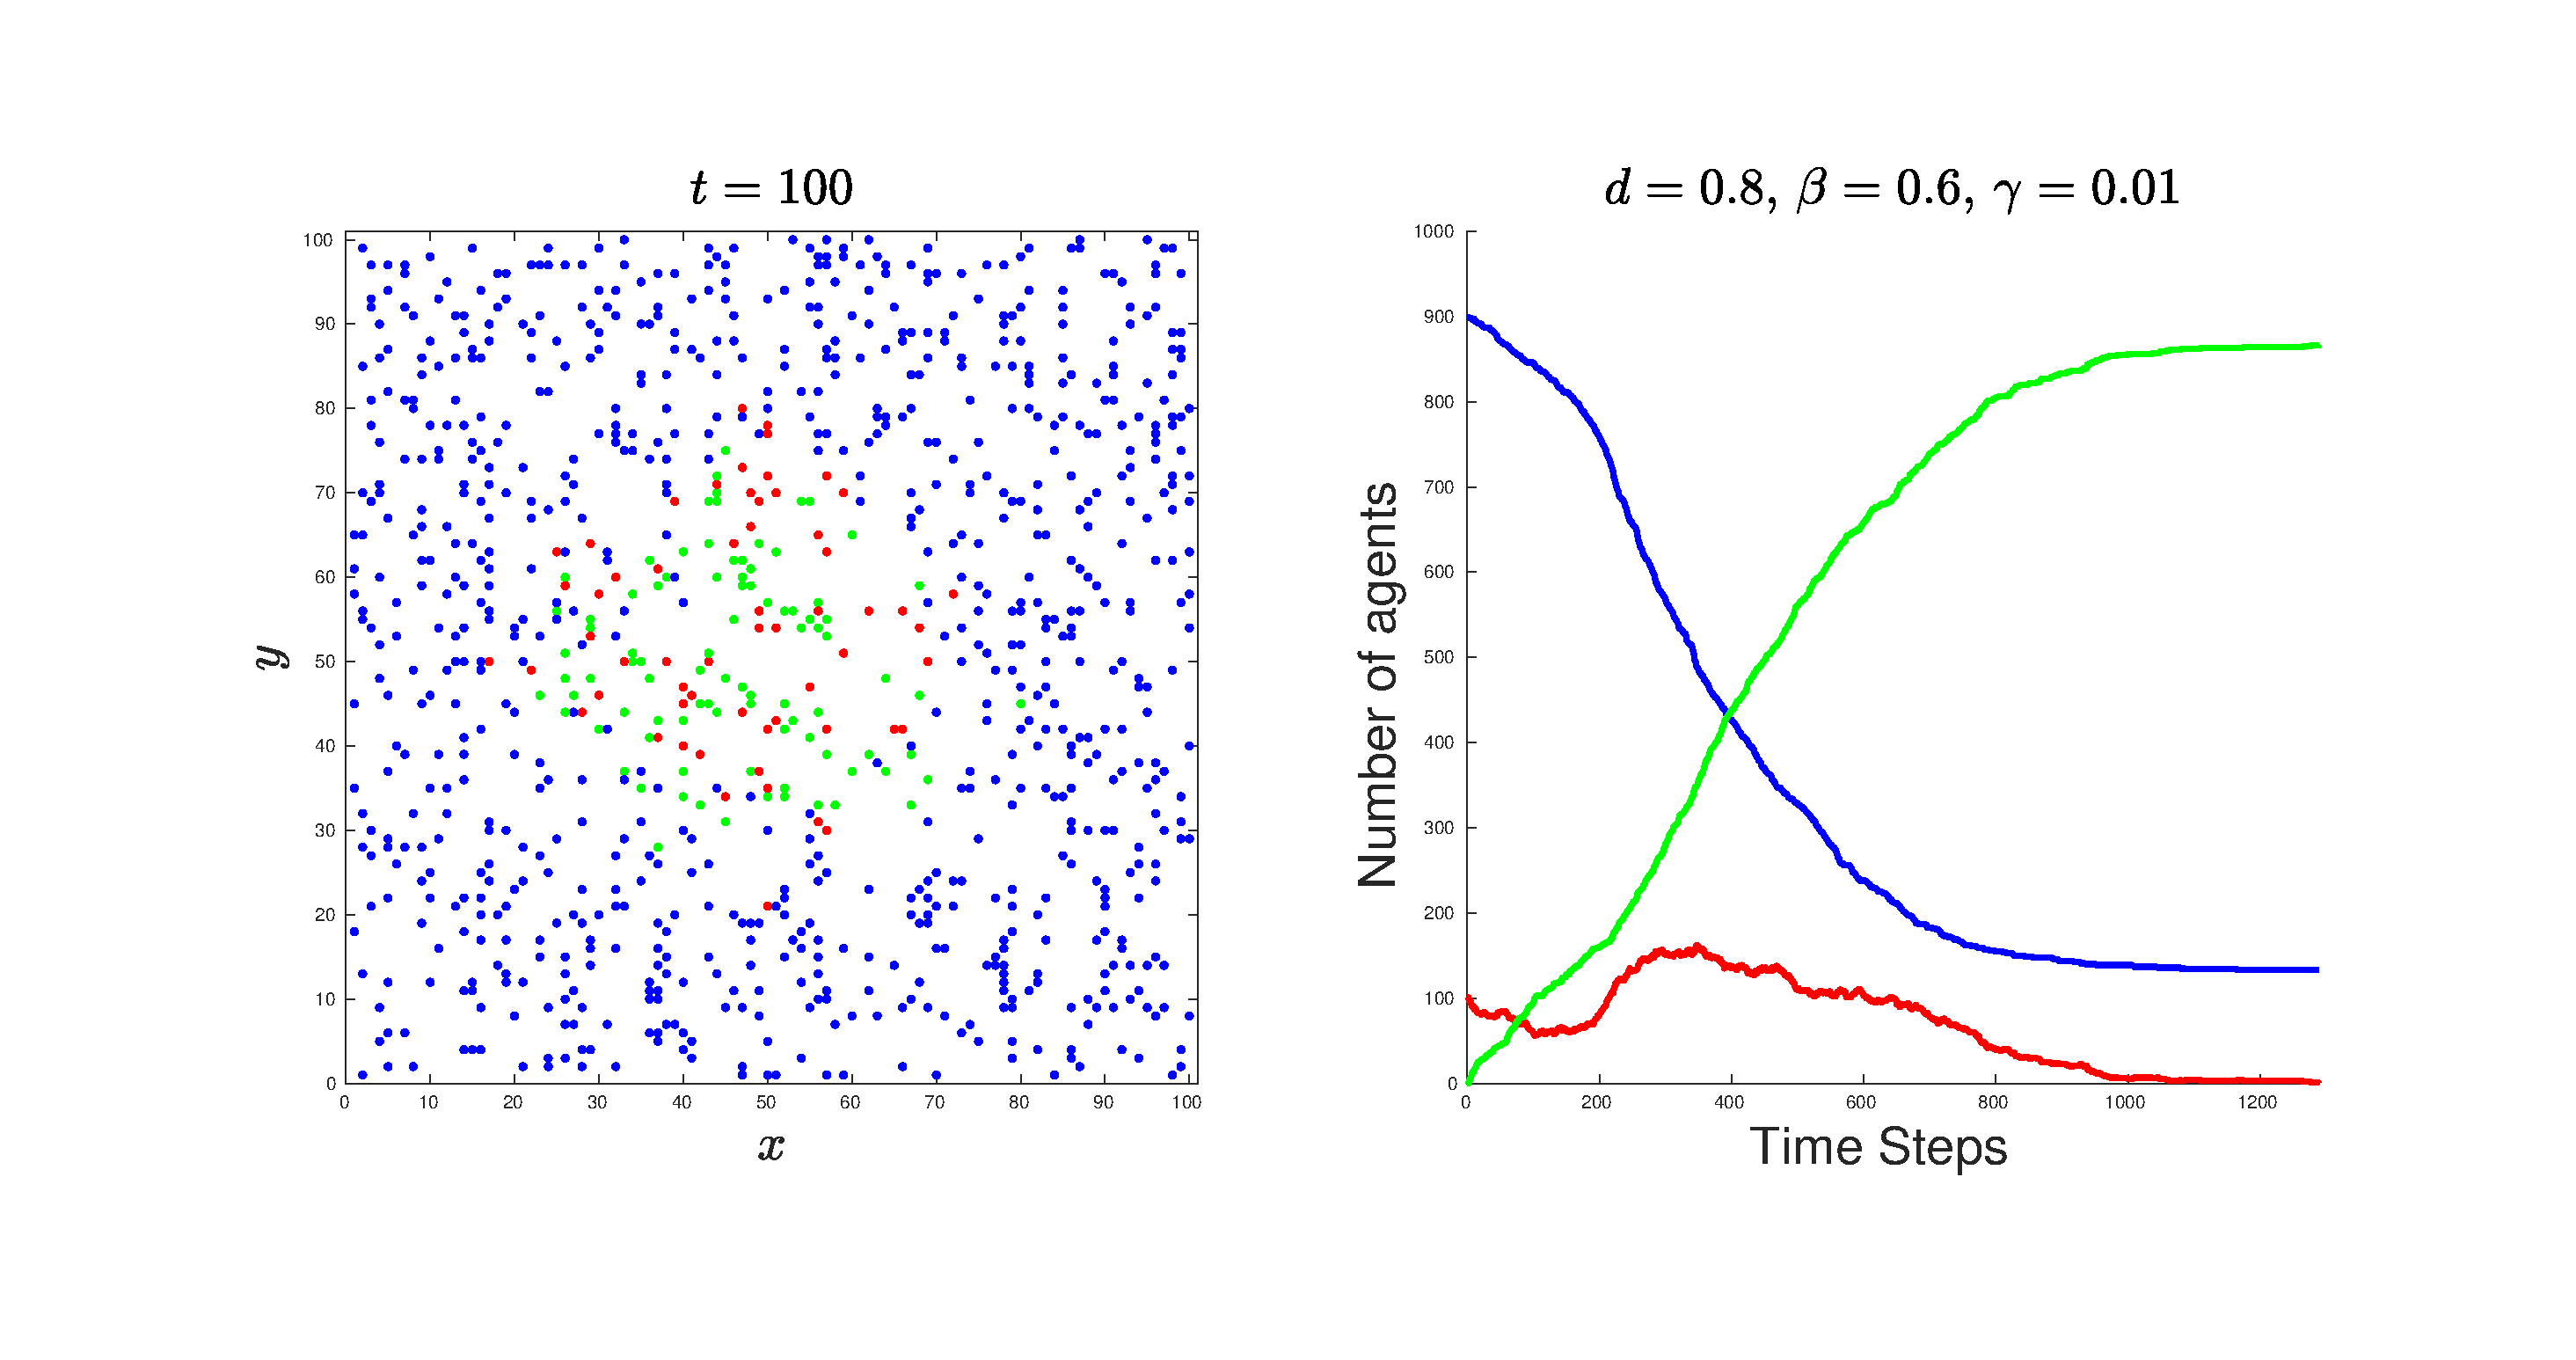
\includegraphics[width=0.9\linewidth]{1_1000_agents}
    \caption{Plot of the proportions of susceptible (blue), infected (red) and recovered (green) individuals in each state over time.}%
    \label{fig:2}
\end{figure}

With the above stated parameters ($d=0.8$, $\beta=0.6$, $\gamma=0.01$), the disease does not spread over the whole population. However over 80\% were infected over time, which could be a very likely scenario of the corona out brake.


\subsection{Probabilistic Health Prediction}

We model partially infected populations as a graph, where each individual (interchangeably called agent) is a node. Edges of this graph model contacts of two agents. We use graph convolution, as explained below, to update our assumptions on the current health state of all individuals.

The definition of a graph convolution~\cite{Kipf2017SemiSupervisedCW} for here is

\begin{equation}
	\label{eq:graph_convolution}
	h_{v_i}^{(l+1)} = \sum_{j\in A(i)} h_{v_j}^{(l)}
\end{equation}

with feature vector $h$ of node $i$ from iteration $(l)$ to $(l+1)$. This formulation is equivalent to the matrix formulation $h^{(l+1)} = A h^{(l)}$ with $A$ as adjacency matrix as shown in \cref{sec:consistency}. We consider here adjacency matrices without diagonal elements.

Our main propagation rule is based on the definition of a graph convolution shown in Eq.~\eqref{eq:graph_convolution} and reads as follows in component notation
\begin{equation}
	h_{v_i, m}^{(l+1)}
	=
	\underbrace{
		\sum_k \textcolor{red}{\frac{\hat{A}_{v_i, k}^{(l)}}{\sum_j \hat{A}_{v_i, j}^{(l)}}} h_{k, m}^{(l)} \textcolor{blue}{\delta_{m, e_I}}
	}_{\text{Graph}}
	+
	\underbrace{
		{(h_{v_i}^{(l)}\cdot T)}_m
	}_{\text{Temporal}}
\end{equation}
with $m$ being the index of the health state.

This propagation rule is based on the following aspects:

\begin{itemize}
	\item The propagation consists of two parts, first the graph contribution and second the temporal contribution. While the former captures the dynamics of infections based on the social contacts between agents, the former ensures that an infected agent heals over time and becomes resistant against the Corona virus.
	\item Each agent $i$ is modeled by $D$ features $h_{v_i}\in\mathbb{R}^D$. Therefore, the feature matrix, $h^{(l)}$, consists of all agents' features at time $(l)$ and is thereby of dimension $N\times D$ where there are $N$ agents in the population and each agent is described by $D$ features. A three dimensional feature space is used, $D=3$, modeling the three possible health states. The unit vectors of this space are interpreted as following:
	\begin{itemize}
		\item $\vec{e}_0$: susceptible state
		\item $\vec{e}_1$: infected state
		\item $\vec{e}_2$: recovered state
	\end{itemize}
	A uniform distribution over these possible states expresses complete uncertainty of the health state of an agent.
	\item Explanation of the graph contribution term:
	\begin{itemize}
		\item A sum over all agents' features $h_{k,m}^{(l)}$ is weighted by the normalised infection-adjusted graph connections as shown in red.
		\item The Kronecker delta, as shown in blue, ensures that only the I feature is added as this is the only one that matters during social contacts between agents.
		\item The infection-adjusted adjacency matrix $\hat{A}$ is constructed from $A$ and $I$ which are the regular continuous adjacency matrix and the infection matrix, respectively. These three quantities are explained in the following:
		\begin{itemize}
			\item The adjacency matrix $A$ is time dependent, $A^{(l)}$, and inferred from data. In our use case, $A_{ij} = \frac{1}{dist(v_i, v_j)+\epsilon}$, hence $A_{ij}$ is large when persons $i$ and $j$ have been in contact. $\epsilon$ serves as regularization for small distances.
			\item The infection matrix is constructed as
			\begin{equation}
				I =
				\begin{pmatrix}
					0     &  0  & 0 \\
					\beta &  0  & \alpha \\
					0     &  0  & 0
				\end{pmatrix}
				=
				(I_{ij})_{i,j}
			\end{equation}
			with $i$ as the index of the host state and $j$ is the index of the contact person state. The states that we consider here are ordered as follows: susceptible, infected, recovered. $\beta$ denotes the probability of infection  after contact (also known as attack rate). $\alpha$ models the probability of being reinfected, which we assume to be zero ($\alpha=0$) based upon current medical \todo{cite!}research.
			\item $\hat{A}$, with $\hat{A}_{ij}\in [0, 1]$, is the adjacency matrix that takes the infection interactions into account and is computed as follows
			\begin{equation}
				\hat{A}_{ij} = A_{ij}\cdot \frac{ h_{v_1}^T I h_{v_2} + h_{v_2}^T I h_{v_1} }{\beta}.
			\end{equation}
			The weighted scalar product of the health states of agents $i$ and $j$ is used to evaluate whether the edge is relevant for the infection dynamics. Only when an infected person and a susceptible have contact, the edge $A_{ij}$ should be considered, otherwise it should be dropped.	The sum in the denominator comes from the fact that both, agent $i$ and $j$, can act as host during a contact. The division by $\beta$ normalises the factor to one to ensure $\hat{A}_{ij} \in [0, 1]$. Since $I$ is not symmetric, $p_a$ is a proper normalization because the sum is in $\{0, p_a\}$. Note that the fraction has the desired properties for pure $S$-, $I$- and $R$-persons.
		\end{itemize}
	\end{itemize}
	\item Explanation of the temporal term:
	\begin{itemize}
		\item The transition of a persons' health state $h_{v_i}^{(l)}$ is determined by the following assumptions:
		\begin{itemize}
			\item A susceptible person always stays susceptible
			\item An infected person has a probability $\gamma$, called recovery rate, to recover. The remaining probability $1-\gamma$ denotes that the person stays sick.
			\item A recovered person could have a probability to be re-infected, but we assume this to be zero. Thus a recovered person always stays recovered.
		\end{itemize}
		\item Thus the temporal transition matrix $T$ is:
		\begin{equation}
			T = 
			\begin{pmatrix}
				1 &     0    & 0      \\
				0 & 1-\gamma & \gamma \\
				0 &     0    & 1      \\
			\end{pmatrix}
		\end{equation}
		\item The temporal update rule based on the health status thus becomes:
		\begin{equation}
			H^{(l+1)} = H^{(l)} T
		\end{equation}
	\end{itemize}
\end{itemize}